\section{The ATLAS Detector}\label{chap:01}

\begin{figure}[H]
    \centering
    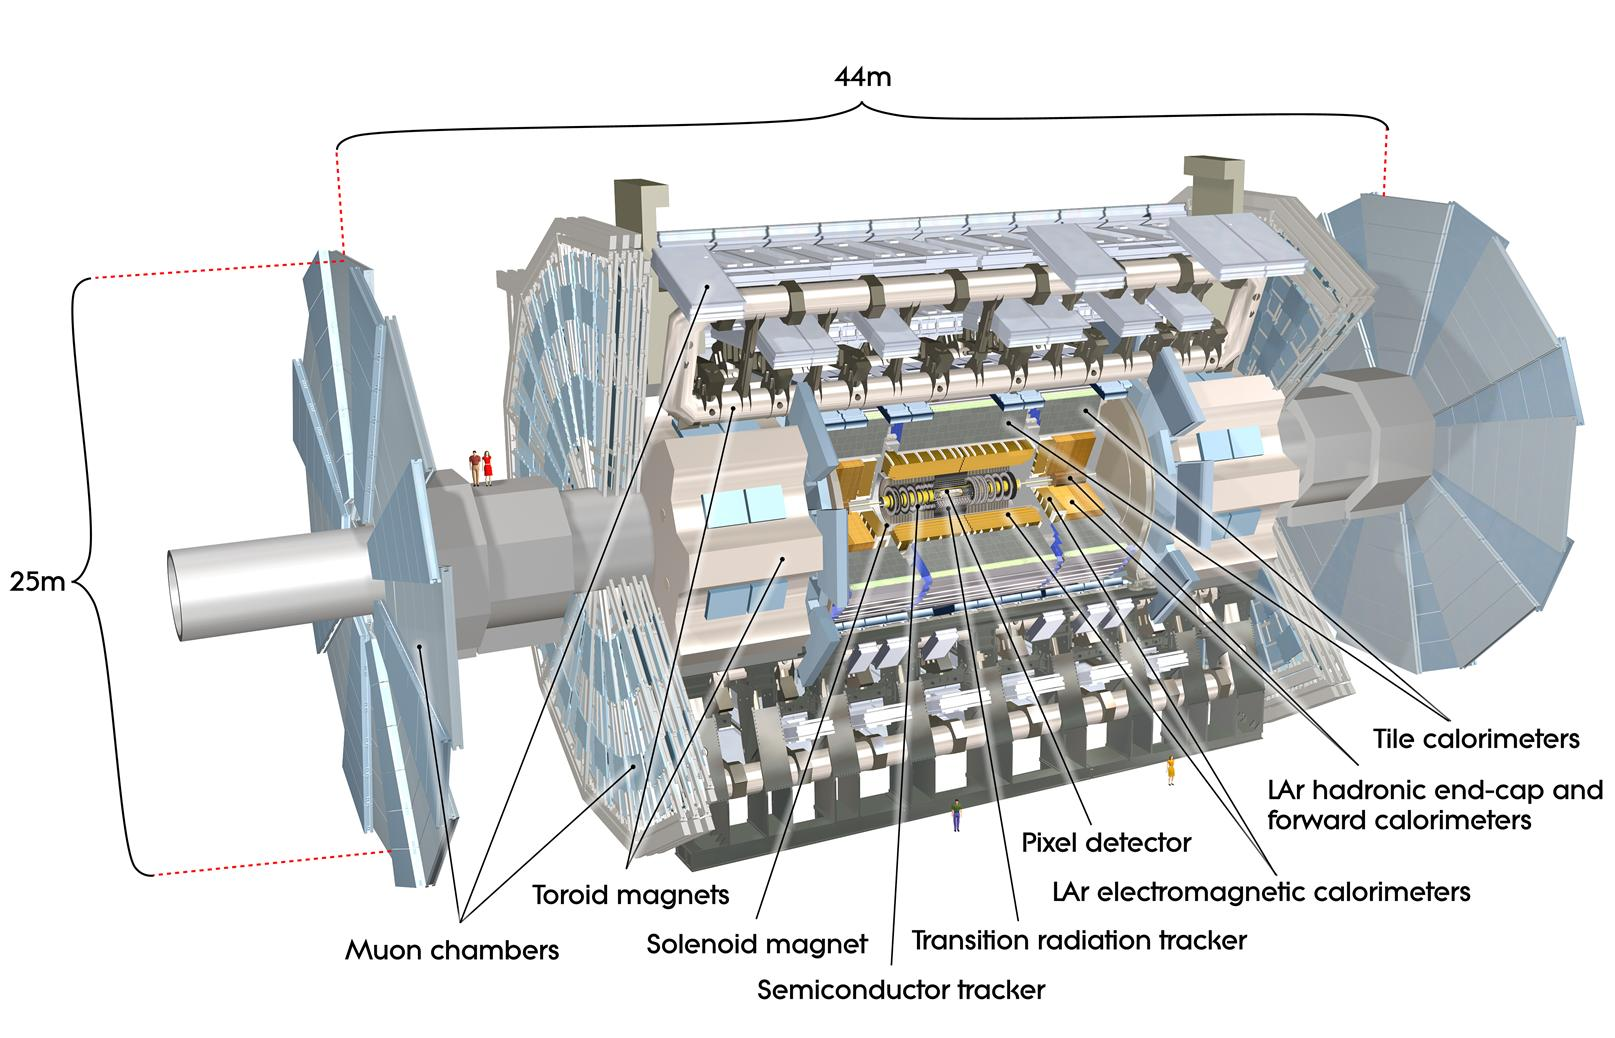
\includegraphics[width=0.75\linewidth]{images/ATLAS_cutout.png}
    \caption{Cutout view of the ATLAS detector \cite{ATLASop}.}
    \label{fig:enter-label}
\end{figure}

The ATLAS detector is a particle detector with a forward-backward symmetric cylindrical geometry and near $4\pi$ coverage in solid angle. Its sub-detectors are arranged in concentric layers around the interaction point. Each layer is specialized to detect or measure particular properties of the particles produced in proton-proton collisions. Following is a description of the major components, moving from the innermost to the outermost layers:

\begin{itemize}
\item \textbf{Inner Detector (ID)}:
\\This subsystem is responsible for tracking charged particles and reconstructing their trajectories. It is immersed in a 2 T solenoidal magnetic field to allow momentum measurement via curvature. It consists of:
\begin{itemize}
\item \textit{Pixel Detector}: Provides the highest granularity and is located closest to the beam pipe. It enables precise vertex reconstruction, crucial for identifying primary and secondary vertices (e.g., from b-quark decays). Operates within $|\eta|<2.5$ range.
\item \textit{Semiconductor Tracker (SCT)}: Composed of silicon microstrip detectors, it offers precision tracking at intermediate radii. Also operates within $|\eta|<2.5$ range.
\item \textit{Transition Radiation Tracker (TRT)}: A straw tube tracker providing continuous tracking and electron identification via transition radiation. Operates within $|\eta|<2$ range.
\end{itemize}

\item \textbf{Calorimeters}:
\\These measure the energy of particles by absorbing them and sampling the resulting showers. They are divided into:
\begin{itemize}
    \item \textit{Electromagnetic Calorimeter (ECAL)}: Built from lead and liquid argon (LAr), it measures energies of electrons and photons with high resolution. Provides coverage up to $|\eta| < 3.2$.
    \item \textit{Hadronic Calorimeter (HCAL)}: Measures energy of hadrons (e.g. pions, kaons). The barrel region uses scintillating tiles and iron absorbers, while endcap and forward regions use copper/tungsten and LAr. Provides coverage up to $|\eta| < 4.9$.
\end{itemize}

\item \textbf{Muon Spectrometer (MS)}:
\\The outermost system, optimized to detect and measure muons. It uses large air-core toroidal magnets and multiple layers of tracking chambers (MDT, CSC) and trigger chambers (RPC, TGC). It provides precise standalone muon momentum measurements. Operates effectively within $|\eta| < 2.7$.

\item \textbf{Magnet Systems}:
\\ATLAS uses two types of magnets:
\begin{itemize}
    \item \textit{Solenoid Magnet}: Surrounds the Inner Detector, producing a 2 T magnetic field for charged particle tracking. Covers the same region as the ID ($|\eta| < 2.5$).
    \item \textit{Toroidal Magnets}: Eight large air-core coils in the barrel and two endcap toroids provide magnetic fields for the Muon Spectrometer. Coverage up to $|\eta| < 2.7$.
\end{itemize}

\item \textbf{Trigger and Data Acquisition System (TDAQ)}:
\\This system selects potentially interesting events from the millions of collisions per second. It consists of a Level-1 hardware trigger and a high-level software trigger system.
\end{itemize}

A hypothetical $Z'$ boson decaying into a top-antitop quark pair ($Z' \rightarrow t\bar{t}$) would lead to different final states rich in leptons, jets, b-jets, and missing transverse energy depending on the decay mode of the subsequent top quark pair ($t\bar{t}$). Charged leptons (electrons or muons) emerging from the decay of the $W$ bosons would first be tracked in the Inner Detector and then deposit energy in the Electromagnetic Calorimeter; muons also traverse the calorimeters and are measured with high precision in the Muon Spectrometer. Jets arising from the hadronization of quarks (including b-quarks) would be reconstructed from energy clusters in the Hadronic Calorimeter and identified as b-jets using precise vertexing in the ID. Neutrinos would pass the detector completely undetected but this would cause an imbalance in transverse momentum ($p_t$) and reflect on the missing energy ($E_{\mathrm{T}}^{\mathrm{miss}}$), calculated from all other reconstructed objects. Together, these detector elements enable us to conduct the full reconstruction and identification of the $Z' \rightarrow t\bar{t}$ decay topology, allowing potential new physics signatures to be distinguished from Standard Model backgrounds.


%----------------------%
%- END OF THE CHAPTER -%
%----------------------%
